%=============================================================
\chapter{Overall Robot Architecture}
\label{chap:robot}
%=============================================================

\section{Hierarchical Structure}

The complete \texttt{Robot} model assembles the sub-models described in the previous chapters into a hierarchical structure. Figure \ref{fig:robot_arch} provides a conceptual overview of the interconnections.

\begin{figure}[H]
  \centering
  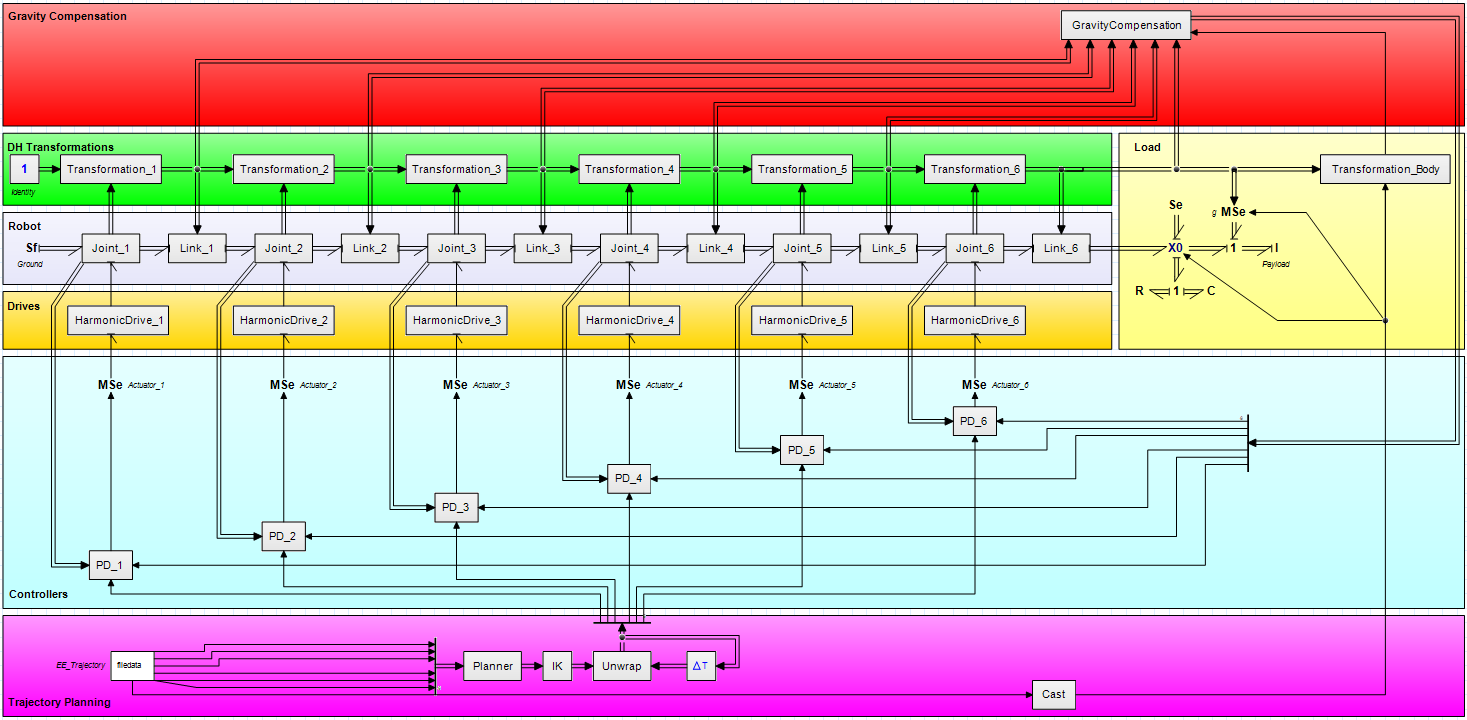
\includegraphics[width=1.0\textwidth]{chapter_robot/figs/robot_struct.png}
  \caption{Full robot architecture.}
  \label{fig:robot_arch}
\end{figure}

\section{Kinematic Chain Assembly}

\subsection{Robot Unit}
The robot comprises identical units consisting of the Joint, Link, Transformation, Harmonic Drive, and a PD controller with gravity compensation, all interconnected sequentially.

\begin{figure}[H]
  \centering
  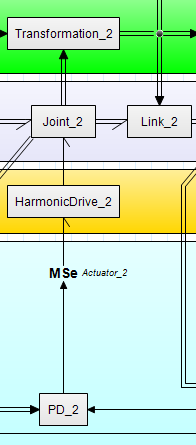
\includegraphics[width=0.3\textwidth]{chapter_robot/figs/robot_unit.png}
  \caption{Robot unit architecture.}
  \label{fig:robot_unit}
\end{figure}

\subsection{Power Bond Chain}

The mechanical power flows from the base (world frame, fixed) through the joints and links in sequence. The base is connected to a \emph{world bond}: a fixed-velocity source that sets the inertial frame velocity to zero ($S_f = 0$ for all six components).

For each link $i = 1,\ldots,6$, the connectivity is defined as:
\begin{center}
  Joint$_i$ (\texttt{twist\_ipp}) $\longrightarrow$ Link$_i$ (\texttt{wrench\_i})
  $\longrightarrow$ Link$_i$ (\texttt{wrench\_ipp}) $\longrightarrow$ Joint$_{i+1}$ (\texttt{twist\_i}).
\end{center}
After Joint$_6$ and Link$_6$, the distal power port terminates either in a free end (zero-force source) or within the payload model.

\subsection{Signal Chain for Transformations}

The absolute transformation chain initializes with $T_0 = I_4$ (the identity matrix, representing the world frame).
\begin{center}
  $T_0$ $\xrightarrow{\text{T\_prev}}$ Transf.$_1$ $\xrightarrow{\text{T\_next}=T_1}$ Transf.$_2$ $\xrightarrow{T_2}$ $\cdots$ $\xrightarrow{T_6}$ GravityTerm.
\end{center}
Each \texttt{Transformation} block also routes \texttt{T\_next} to the \texttt{MSe} element of the corresponding \texttt{Link} block (for gravity vector orientation) and to the 3D visualization.


\section{Global Causality Analysis}

The Link sub-model acts as an \textbf{I-field} in integral causality; therefore, its outputs at both ports are flows. This matches the causality of the Joint sub-model, which instead outputs effort from both ports. 

Consequently, the Joint block imposes the effort onto the robot chain, while the Links (representing the inertias) define the resulting velocities in response to this effort. 

To manage these computational constraints: 
\begin{itemize}
  \item The world bond imposes velocity (effort-out causality at the base).
  \item At the base, a source of flow ($S_f = 0$) simulates a stationary ground.
  \item At the end-effector (a Link), it is possible to attach either a source of effort to simulate a contact force, or an additional inertia with gravity to simulate a load.
  \item The harmonic drive outputs an effort, simulating a mechanical transmission. 
  \item The motor driving the shaft is simulated as a source of effort.
\end{itemize}

Moreover, the non-linear C-element within the harmonic drive retains integral causality. No derivative causality is present in the final assembled model, ensuring the numerical stability of the constrained integration via BDF solvers. 

\section{Payload Model}

A point-mass payload $m_{\text{load}}$ attached at the end-effector (the distal port of Link 6) is modeled as an additional \texttt{Link} block with:
\begin{itemize}
  \item $m = m_{\text{load}}$.
  \item $J = J_{\text{load}}$.
  \item $r_{Gp} = [0,0,0]^T$ (mass concentrated at the attachment point).
\end{itemize}

Gravity is also applied to its center of mass, which corresponds to the origin of the end-effector. This gravity vector is properly rotated according to the DH transformation of the end-effector frame. 

Lastly, to ensure a rigid connection between the final link and the payload, a zero-junction with a velocity constraint is employed in the exact same manner as in the Joint sub-model. 

\begin{figure}[H]
  \centering
  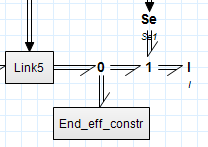
\includegraphics[width=0.4\textwidth]{chapter_robot/figs/load.png}
  \caption{Mass load architecture.}
  \label{fig:load_arch}
\end{figure}


\section{3-D Visualization}

The 20-sim 3-D Mechanics toolbox receives the pose signals (\texttt{pose\_abs}) and the rotation matrices from each \texttt{Transformation} block. STL bodies based on the UR5 model are utilized to represent each link. These bodies are positioned and oriented dynamically according to the offset positions and rotation matrices computed within the transformation blocks. 

\begin{figure}[H]
  \centering
  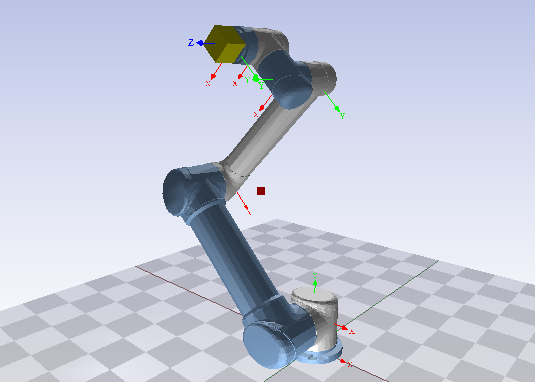
\includegraphics[width=0.8\textwidth]{chapter_robot/figs/stl1.png}
  \caption{Robot 3D visualization.}
  \label{fig:robot_visu}
\end{figure}